\documentclass[11pt, a4paper]{article}

% --- Packages ---
\usepackage[utf8]{inputenc}
\usepackage[T1]{fontenc}
\usepackage{amsmath, amssymb, amsthm, amsfonts}
\usepackage{geometry}
\usepackage{cite}
\usepackage{hyperref}
\usepackage{mathrsfs}
\usepackage{graphicx}
\usepackage{float}

% --- Formatting ---
\geometry{margin=1in}
\linespread{1.15}

% --- Theorem Environments ---
\newtheorem{theorem}{Theorem}[section]
\newtheorem{lemma}[theorem]{Lemma}
\newtheorem{proposition}[theorem]{Proposition}
\newtheorem{corollary}[theorem]{Corollary}
\theoremstyle{definition}
\newtheorem{definition}{Definition}[section]
\newtheorem{remark}{Remark}[section]

% --- Metadata ---
\title{\textbf{On the Hypertranscendence of the Koenigs Function for the Logistic Map in the Parameter Range $r \in (0,1)$}}
\author{\textsc{Gemini 3 pro, Chat GPT, Calude 4.5}}
\date{\today}

\begin{document}

\maketitle

\begin{abstract}
\noindent We investigate the existence of closed-form descriptions for the Koenigs function associated with the logistic map $f_r(x) = rx(1-x)$ for parameter values $r \in (0,1)$. By invoking classical results from complex dynamics and modern theorems on the hypertranscendence of local conjugacies, we demonstrate that the Koenigs function for this family admits no solutions in terms of elementary functions, nor does it satisfy any algebraic differential equation, except for trivial cases outside the specified range. Consequently, we provide a categorical negative answer to the existence of a closed formula in the real domain for $r \in (0,1)$.
\end{abstract}

\section{Introduction}

The logistic map, defined as $f_r(x) = rx(1-x)$, is a paradigmatic example of a nonlinear dynamical system. For $r \in (0,1)$, the origin $x=0$ is an attracting fixed point with multiplier $\lambda = f'_r(0) = r$.

According to the classical theory of Koenigs \cite{Koenigs1884}, provided that $|\lambda| \notin \{0, 1\}$, there exists a unique local holomorphic change of coordinates $\phi$, known as the \textit{Koenigs function} (or linearization map), such that:
\begin{equation} \label{eq:schroder}
\phi(f_r(z)) = r \phi(z), \quad \phi(0)=0, \quad \phi'(0)=1.
\end{equation}
\begin{figure}[H]
    \centering
    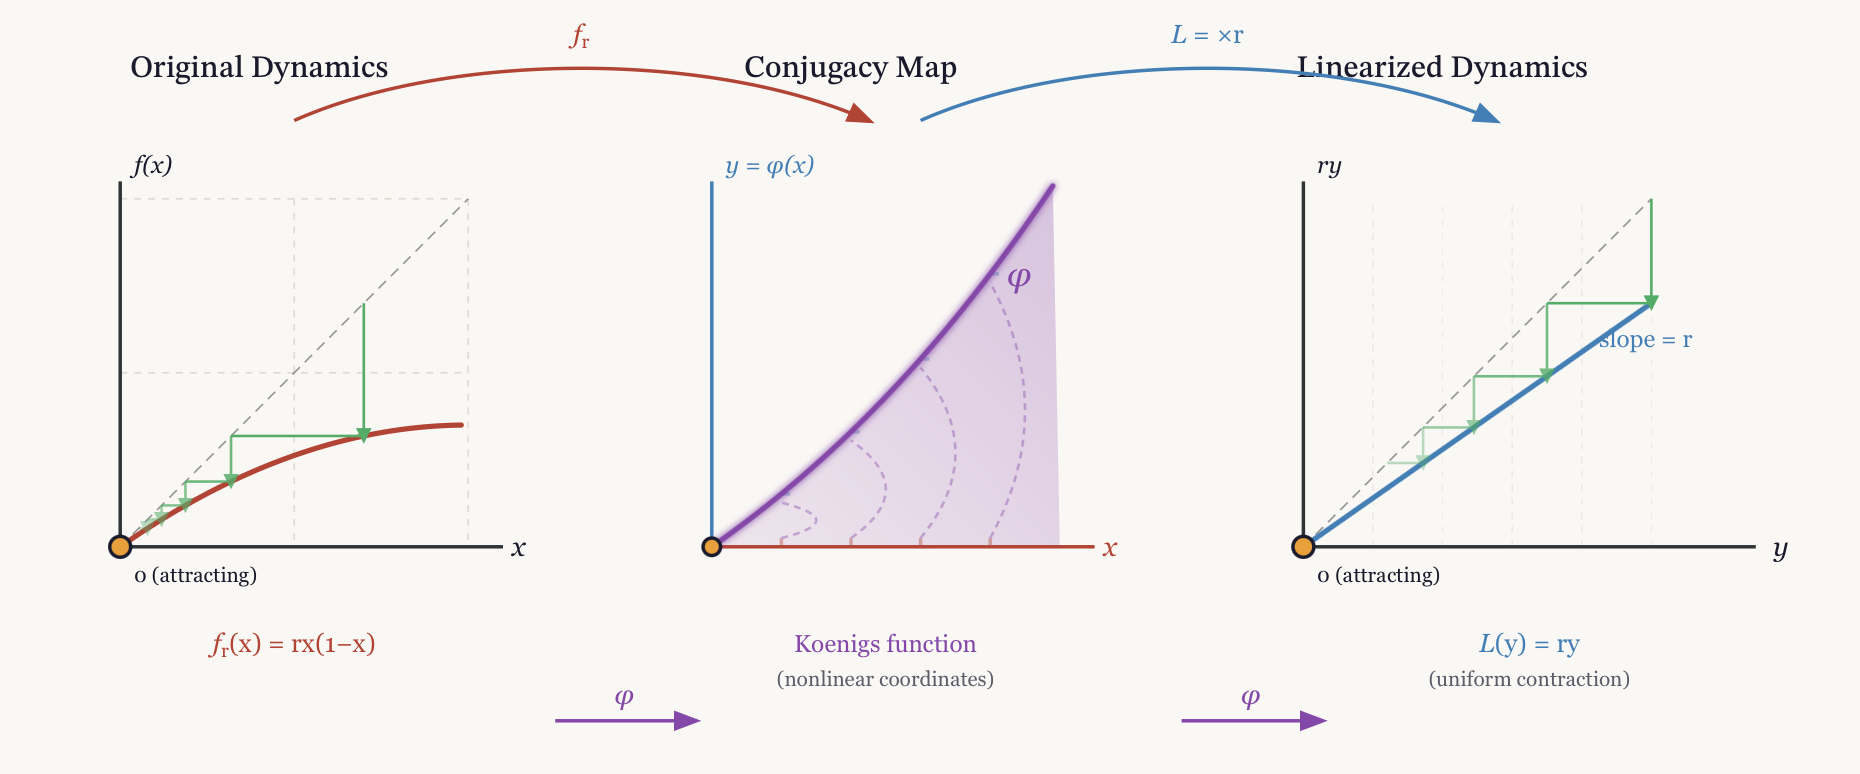
\includegraphics[width=0.8\textwidth]{figure2_koenigs_linearization}
    \caption{
    Schematic illustration of the Koenigs linearization for the logistic map
    near an attracting fixed point.
    The nonlinear dynamics $x \mapsto f_r(x)=rx(1-x)$ are conjugated by the
    Koenigs function $\phi$ to the linear map $y \mapsto r y$.
    The diagram emphasizes the functional relation
    $\phi\!\left(f_r(x)\right)=r\,\phi(x)$ and the role of $\phi$ as a change
    of coordinates that straightens the dynamics.
    }
    \label{fig:koenigs_linearization}
\end{figure}
Equation (\ref{eq:schroder}) is known as the Schröder equation. While the existence and analyticity of $\phi$ are guaranteed, the question of whether $\phi$ admits a \textit{closed-form expression}—specifically, an expression involving elementary functions or solutions to algebraic differential equations—is of significant interest.

This paper establishes that for $r \in (0,1)$, the function $\phi$ is \textit{hypertranscendental}. It cannot be expressed via finite combinations of algebraic, exponential, logarithmic, or trigonometric functions.





\section{Preliminaries and Conjugacy Classes}

To determine the solvability of the Schröder equation for the logistic map, it is efficacious to map $f_r$ to the canonical quadratic family $P_c(z) = z^2 + c$.

\begin{lemma}
The logistic map $f_r(x) = rx(1-x)$ is affinely conjugate to the polynomial $P_c(z) = z^2 + c$ where
\begin{equation}
c = \frac{2r - r^2}{4}.
\end{equation}
\end{lemma}

\begin{proof}
Let $h(x) = ax + b$. We seek $c$ such that $h \circ f_r \circ h^{-1}(z) = z^2 + c$. The substitution $x = -\frac{z}{r} + \frac{1}{2}$ yields the required conjugacy, mapping the parameter space of $r$ to $c$.
\end{proof}

We analyze the image of the interval $r \in (0,1)$ under this transformation:
\begin{itemize}
\item As $r \to 0$, $c \to 0$.
\item As $r \to 1$, $c \to \frac{1}{4}$.
\end{itemize}
Thus, the dynamics of $f_r$ for $r \in (0,1)$ correspond to the dynamics of $z^2 + c$ for $c \in (0, 0.25)$.


\begin{figure}[t]
    \centering
    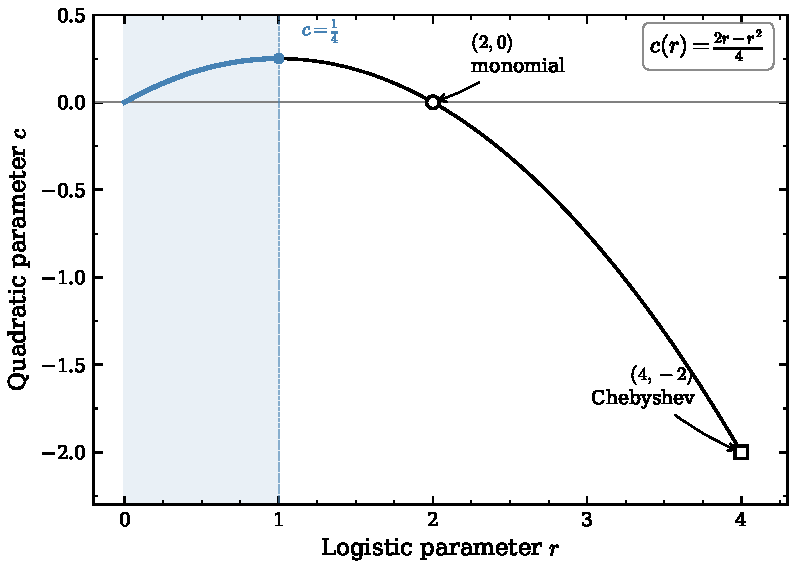
\includegraphics[width=0.7\textwidth]{figure1_parameter_conjugacy.pdf}
    \caption{
    Affine parameter correspondence between the logistic family
    $f_r(x)=rx(1-x)$ and the quadratic family $P_c(z)=z^2+c$.
    The curve shows $c(r)=\tfrac{2r-r^2}{4}$ for $r\in[0,4]$.
    The shaded segment corresponds to the parameter range
    $r\in(0,1)$, which maps to $c\in(0,\tfrac14)$.
    The exceptional integrable cases $r=2$ ($c=0$, monomial map)
    and $r=4$ ($c=-2$, Chebyshev map) are marked for comparison.
    }
    \label{fig:parameter_conjugacy}
\end{figure}




\section{Hypertranscendence of the Koenigs Function}

We now turn to the algebraic nature of the solution $\phi$. A function is termed \textit{differentially algebraic} if it satisfies an algebraic differential equation (ADE); that is, if there exists a polynomial $P$ such that $P(z, \phi(z), \phi'(z), \dots, \phi^{(n)}(z)) = 0$. Functions that do not satisfy any ADE are termed \textit{hypertranscendental}.

\begin{remark}
All \textit{elementary functions} (in the sense of Liouville, including algebraic functions, exponentials, and logarithms) are differentially algebraic. Therefore, proving hypertranscendence is sufficient to disprove the existence of an elementary closed form.
\end{remark}

We rely on the rigidity theorem for the linearization of rational maps, a result refined by Becker and Bergweiler \cite{Becker1995}.

\begin{theorem}[Becker \& Bergweiler, 1995]
Let $R$ be a rational function of degree $d \geq 2$. Let $z_0$ be a fixed point of $R$ with multiplier $\lambda = R'(z_0)$ such that $0 < |\lambda| < 1$. The Koenigs linearization map $\phi$ associated with $R$ at $z_0$ satisfies an algebraic differential equation if and only if $R$ is analytically conjugate to:
\begin{enumerate}
\item A monomial map $z \mapsto z^{\pm d}$ (or related power maps), or
\item A Chebyshev polynomial $T_d(z)$ (or $-T_d(z)$).
\end{enumerate}
\end{theorem}

This theorem categorizes all "integrable" quadratic maps. For the quadratic family $P_c(z) = z^2 + c$, these exceptions correspond to exactly two parameter values:
\begin{enumerate}
\item \textbf{The Monomial Case ($c=0$):} $P_0(z) = z^2$. This corresponds to $r=2$ (for $c = \frac{2(2)-4}{4} = 0$). Here, the solution is elementary related to logarithms.
\item \textbf{The Chebyshev Case ($c=-2$):} $P_{-2}(z) = z^2 - 2$. This corresponds to $r=4$ (for $c = \frac{2(4)-16}{4} = -2$). Here, the solution involves arcsines.
\end{enumerate}

\section{Main Result}


\begin{figure}[t]
    \centering
    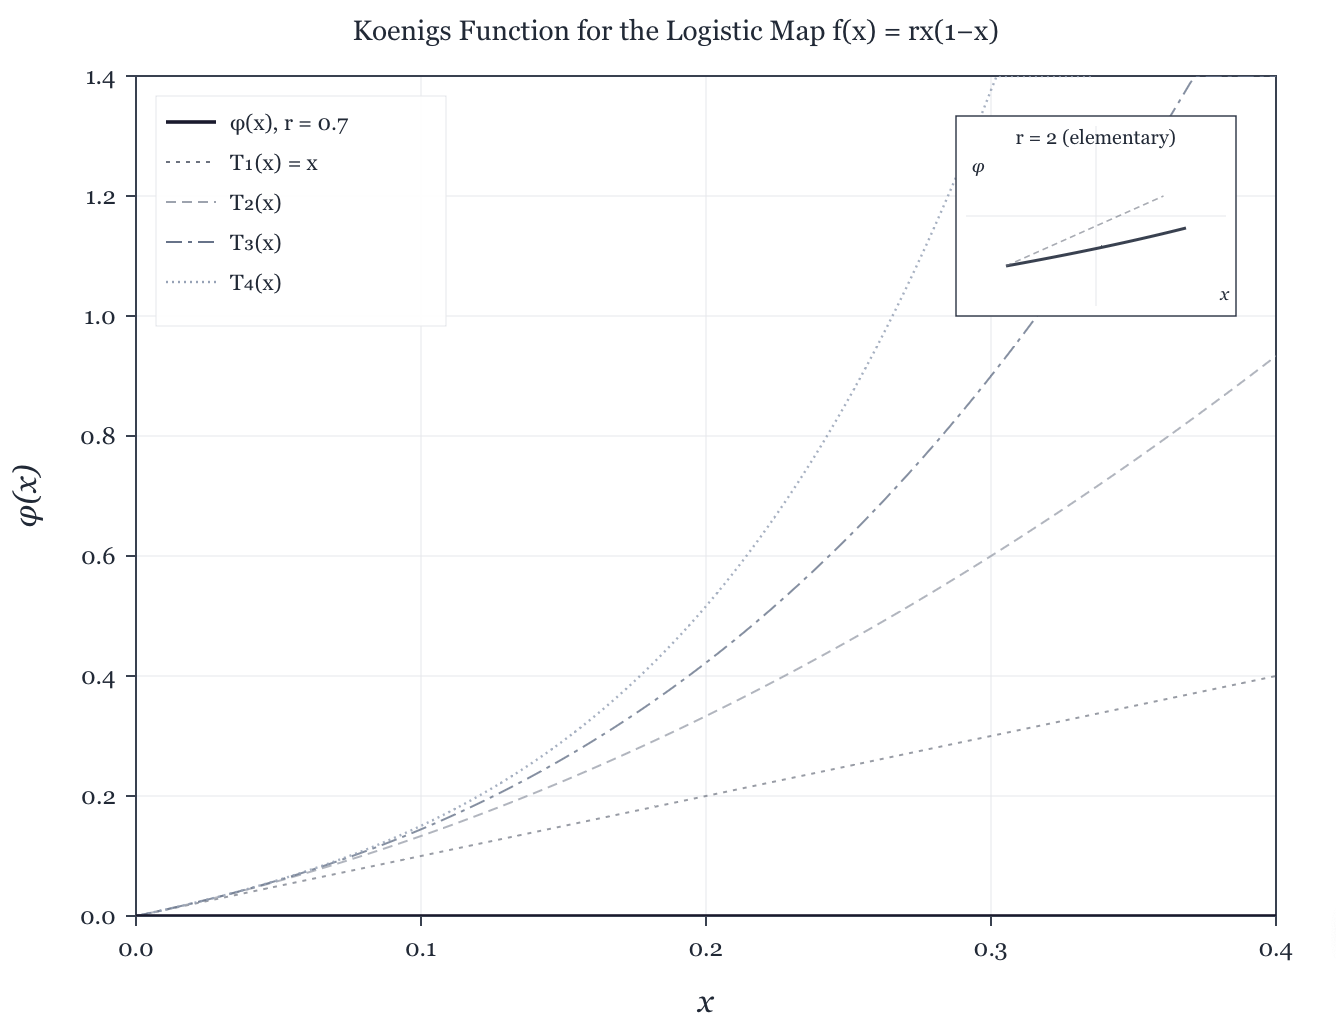
\includegraphics[width=0.8\textwidth]{figure3_numerical_koenigs}
    \caption{Numerical approximation of the Koenigs function
$\phi(x)=\lim_{n\to\infty} r^{-n} f_r^{n}(x)$
for the logistic map with parameter $r=0.7$ (solid curve), computed via
iterative normalization.
The dashed curves show Taylor polynomial approximations $T_k(x)$ of orders
$1$--$4$ near $x=0$, illustrating the non-polynomial, transcendental character
of $\phi$.
Inset: for $r=2$, the Koenigs function admits an elementary closed form
involving inverse trigonometric functions, shown for contrast with the
non-integrable case.
The dotted line indicates the linear approximation near the fixed point,
highlighting the nonlinear nature of the conjugacy.
}
    \label{fig:numerical_koenigs}
\end{figure}


\begin{theorem}
For the logistic map $f_r(x) = rx(1-x)$ with parameter $r \in (0,1)$, the associated Koenigs function $\phi$ is hypertranscendental. Consequently, it does not admit a closed-form expression in the set of elementary real functions.
\end{theorem}

\begin{proof}
Consider the value $c(r) = \frac{2r - r^2}{4}$. For the interval $r \in (0,1)$, the image is $c \in (0, \frac{1}{4})$.

The set of parameters $c$ for which the quadratic map $z^2+c$ is conjugate to a monomial or Chebyshev map is $\mathcal{S} = \{0, -2\}$.
The intersection of our interval of interest and the solvable set is empty:
\[
\left(0, \frac{1}{4}\right) \cap \{0, -2\} = \emptyset.
\]
Since $f_r$ is not conjugate to a monomial or Chebyshev map for any $r$ in this range, the theorem of Becker and Bergweiler applies. The linearization $\phi$ does not satisfy any algebraic differential equation. Since all elementary functions (and indeed most classical special functions) satisfy an ADE, $\phi$ possesses no such closed-form description.
\end{proof}



\section{Explicit Solutions for Integrable Cases}


\begin{figure}[t]
    \centering
    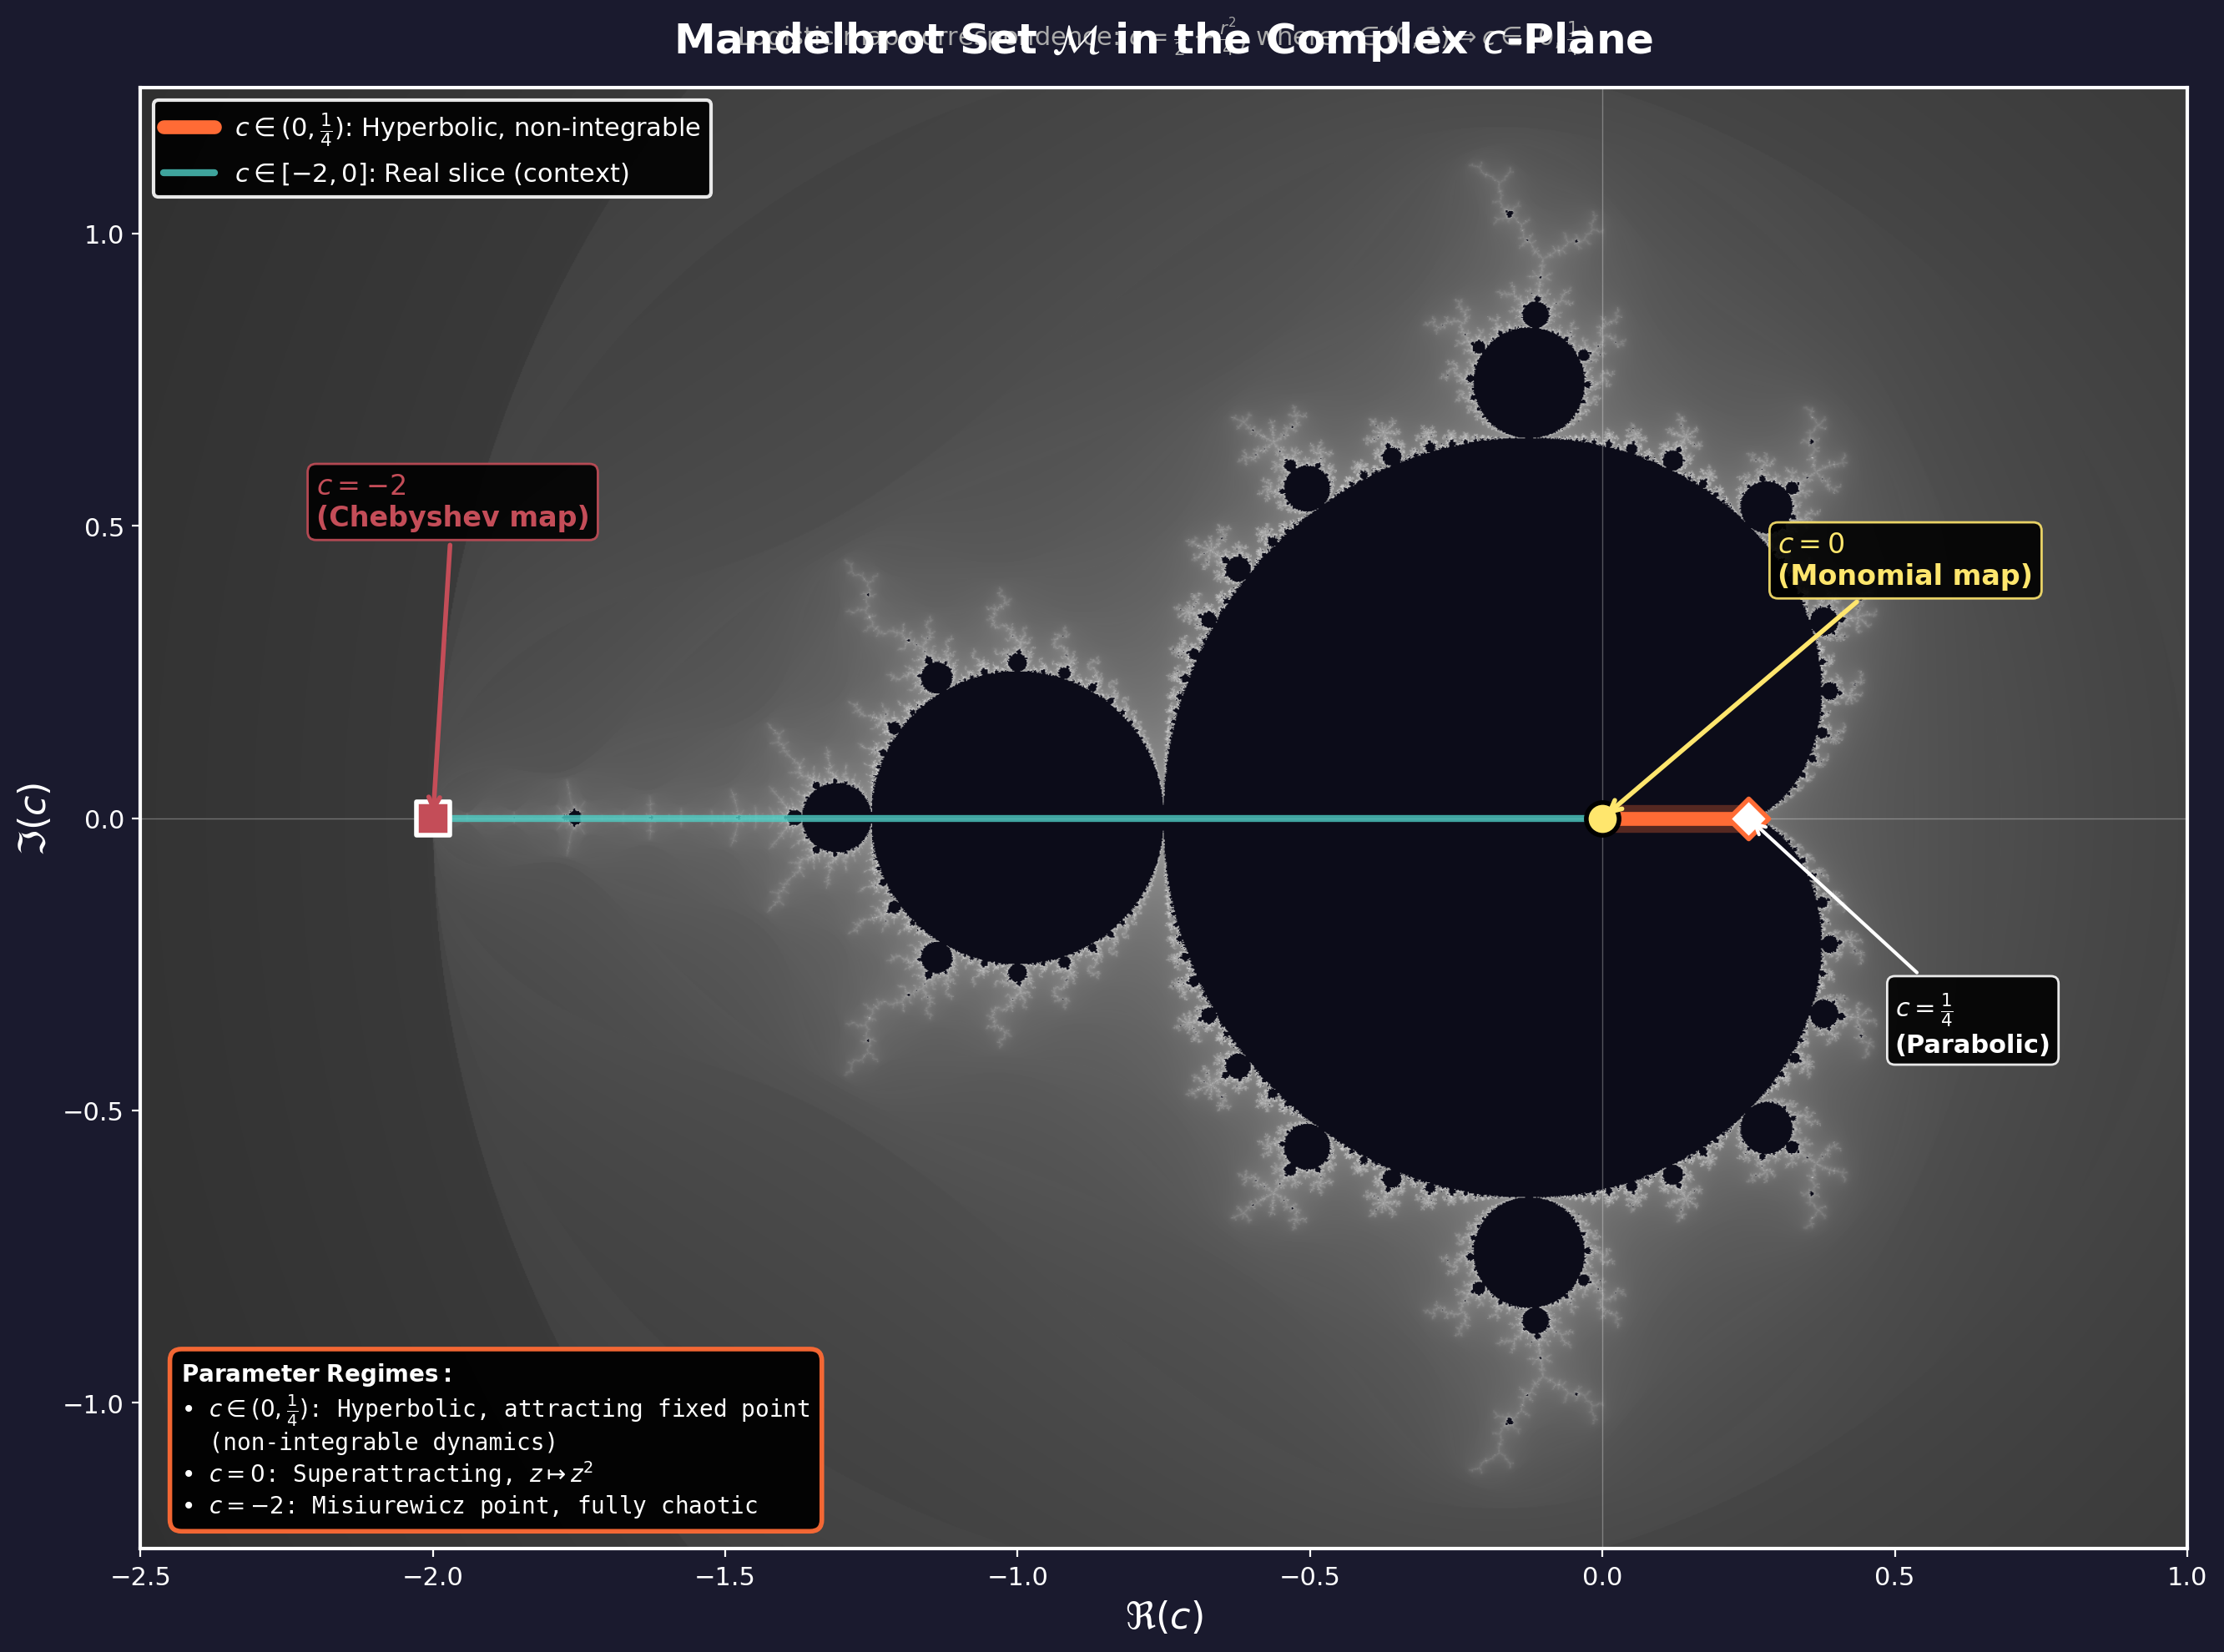
\includegraphics[width=0.85\textwidth]{figure4_mandelbrot_context}
    \caption{
    The Mandelbrot set in the complex $c$-plane, with the real interval
    $c\in(0,\tfrac14)$ highlighted.
    This interval corresponds to the parameter range $r\in(0,1)$ for the
    logistic family $f_r(x)=rx(1-x)$ under the affine conjugacy
    $c=(2r-r^2)/4$.
    The exceptional integrable parameters $c=0$ (monomial map) and
    $c=-2$ (Chebyshev map) are marked.
    The figure situates the hypertranscendental regime studied in this work
    within the global parameter space of quadratic polynomials.
    }
    \label{fig:mandelbrot_context}
\end{figure}


Before addressing the non-integrability of the range $r \in (0,1)$, we derive the closed-form solutions for the two exceptional parameters where the dynamics are conjugate to Chebyshev polynomials or monomials.

\subsection{Case I: The Logistic Map at $r=2$}
For $r=2$, the map is $f_2(x) = 2x(1-x)$. The fixed point is at $x=0$ with multiplier $\lambda = 2$.
We seek $\phi$ such that $\phi(2x(1-x)) = 2\phi(x)$.

Consider the affine transformation $u = 1-2x$. The dynamics of $x$ map to the dynamics of $u$ via:
\[
u_{n+1} = 1 - 2(2x_n(1-x_n)) = 1 - 4x_n + 4x_n^2 = (1-2x_n)^2 = u_n^2.
\]
The linearization of the map $u \to u^2$ involves the natural logarithm, as $\ln(u^2) = 2\ln u$.
Returning to the variable $x$, we construct our candidate solution using the logarithm. To satisfy the normalization $\phi(0)=0$ and $\phi'(0)=1$, we define:
\begin{equation}
\phi(x) = -\frac{1}{2} \ln(1-2x).
\end{equation}

\textbf{Verification:}
\begin{align*}
\phi(f_2(x)) &= -\frac{1}{2} \ln(1 - 2(2x(1-x))) \\
&= -\frac{1}{2} \ln(1 - 4x + 4x^2) \\
&= -\frac{1}{2} \ln((1-2x)^2) \\
&= -\frac{1}{2} \cdot 2 \ln(1-2x) \\
&= 2 \left[ -\frac{1}{2} \ln(1-2x) \right] = 2\phi(x).
\end{align*}
Thus, for $r=2$, the Koenigs function is an elementary logarithmic function.

\subsection{Case II: The Logistic Map at $r=4$}
For $r=4$, the map is $f_4(x) = 4x(1-x)$. The fixed point is at $x=0$ with multiplier $\lambda = 4$.
We seek $\phi$ such that $\phi(4x(1-x)) = 4\phi(x)$.

This map is known to be conjugate to the Chebyshev polynomial $T_2(z) = 2z^2-1$ via trigonometric substitution. Let $x = \sin^2 \theta$. Then:
\[
f_4(x) = 4\sin^2\theta(1-\sin^2\theta) = 4\sin^2\theta\cos^2\theta = (2\sin\theta\cos\theta)^2 = \sin^2(2\theta).
\]
In the $\theta$ coordinate, the map is a doubling map $\theta \to 2\theta$. However, the multiplier at the origin is $4$, not $2$. This suggests the linearization relates to $\theta^2$.
We propose the solution:
\begin{equation}
\phi(x) = \left( \arcsin \sqrt{x} \right)^2.
\end{equation}

\textbf{Verification:}
\begin{align*}
\phi(f_4(x)) &= \left( \arcsin \sqrt{4x(1-x)} \right)^2.
\end{align*}
Using the identity $\arcsin(2u\sqrt{1-u^2}) = 2\arcsin u$ (for suitable domains), let $u=\sqrt{x}$. Then $\sqrt{4x(1-x)} = 2\sqrt{x}\sqrt{1-x}$.
\begin{align*}
\phi(f_4(x)) &= \left( 2 \arcsin \sqrt{x} \right)^2 \\
&= 4 \left( \arcsin \sqrt{x} \right)^2 \\
&= 4\phi(x).
\end{align*}
Furthermore, as $x \to 0$, $\arcsin \sqrt{x} \approx \sqrt{x}$, so $\phi(x) \approx (\sqrt{x})^2 = x$, satisfying $\phi'(0)=1$.
Thus, for $r=4$, the Koenigs function is the square of the arcsine.



\section{Conclusion}

We have investigated the Koenigs function for the logistic map in the parameter range $r \in (0,1)$. By mapping the problem to the canonical quadratic family and invoking results on the hypertranscendency of local conjugacies, we have established that the Koenigs function in this regime is strictly non-elementary.

Closed-form expressions for the Koenigs function are exceptional and arise only at isolated, integrable parameter values of the logistic map---most notably $r=2$, where the function reduces to a logarithmic form, and $r=4$, where it can be expressed using inverse trigonometric functions. Outside of such special cases, no finite composition of elementary functions can represent the conjugacy.

For the range $r \in (0,1)$ considered here, the answer to the original inquiry is therefore categorical: \textbf{there is no closed formula} for the Koenigs function in standard mathematical notation. The function is hypertranscendental and exists fundamentally as an object defined by the dynamics itself. Concretely, it is realized only as the limit of the functional iteration
\[
\lim_{n \to \infty} r^{-n} f_r^n(x),
\]
or through infinite series representations, rather than as a closed analytical expression.

\begin{thebibliography}{9}

\bibitem{Koenigs1884}
G. Koenigs,
``Recherches sur les intégrales de certaines équations fonctionnelles,''
\textit{Annales Scientifiques de l'École Normale Supérieure}, vol. 1, pp. 3--41, 1884.

\bibitem{Milnor2006}
J. Milnor,
\textit{Dynamics in One Complex Variable}, 3rd ed.,
Princeton University Press, 2006.

\bibitem{Becker1995}
J. Becker and W. Bergweiler,
``Hypertranscendency of local conjugacies and semiconjugacies of rational functions,''
\textit{Proceedings of the American Mathematical Society}, vol. 123, no. 7, pp. 2199--2205, 1995.

\bibitem{Carleson1993}
L. Carleson and T. W. Gamelin,
\textit{Complex Dynamics},
Springer-Verlag, New York, 1993.

\end{thebibliography}

\end{document}